\documentclass[a4paper,spanish]{article}

\usepackage[T1]{fontenc}
\usepackage[utf8]{inputenc}
\usepackage{babel}
\usepackage{lmodern}
\usepackage{fullpage}
\usepackage{enumerate}

\usepackage{tabularx}
\usepackage{graphicx}
\usepackage{amsthm}
\usepackage{amsmath}
\usepackage{amssymb}
\usepackage{delarray}
\pagenumbering{arabic}
\decimalpoint
\graphicspath{ {./images/} }

%% Document Header
\title{Entrega Clase 2 - Estadística}
\author{Alejandro Uribe}
\date{Octubre 2022}

\begin{document}
\maketitle
\section*{Enunciado}

Sea $X$ una variable aleatoria con la siguiente función de distribución:

\[
    F_X(x) =
    \begin{cases}
        0   & \text{$x<1$}          \\
        0.4 & \text{$1 \leq x < 2$} \\
        0.7 & \text{$2 \leq x < 5$} \\
        1   & \text{$x \geq 5$}     \\
    \end{cases}
\]

\begin{enumerate}
    \item Graficar $F_X(x)$

          \begin{figure}[h]
              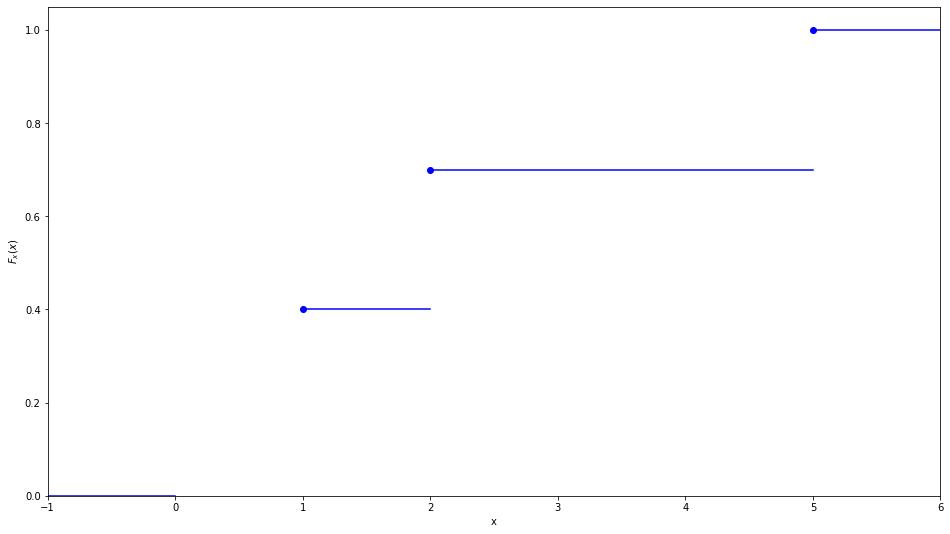
\includegraphics[width=10cm]{Fxx}
              \centering
          \end{figure}



    \item Hallar el rango $R_x$ y la función de probabilidad de $X$, $p_x(x)$.

          $R_x$ está dado por el conjunto de puntos para los cuales la función de probabilidad puntual es diferente de cero, es decir,
          \begin{align*}
              R_x & = \left\{ x \in \mathbf{R}: p_x(x) \neq 0 \right\} \\
              R_x & = \left\{ 1,2,3,4,5 \right\}
          \end{align*}

          La función de probabilidad de $X$ se define como: $p_x(x) = P(X=x) = F_X(x) - F_X(x^-)$. Notar que para el intervalo $2 \leq x < 5$ la probabilidad es la misma.
          \begin{itemize}
              \item $p_x(1) = P(X=1) = F_X(1) - F_X(1^-) = 0.4 - 0.0 = 0.4$
              \item $p_x(2) = P(X=2) = F_X(2) - F_X(2^-) = 0.7 - 0.4 = 0.3$
              \item $p_x(3) = P(X=2) = 0.3$
              \item $p_x(4) = P(X=2) = 0.3$
              \item $p_x(5) = P(X=5) = F_X(5) - F_X(5^-) = 1.0 - 0.7 = 0.3$
          \end{itemize}

          Los resultados anteriores se muestran en la siguiente tabla:

          \begin{tabularx}{0.8\textwidth} {
              >{\centering\arraybackslash}X
              | >{\centering\arraybackslash}X
              |>{\centering\arraybackslash}X
              >{\centering\arraybackslash}X
              >{\centering\arraybackslash}X
              | >{\centering\arraybackslash}X }

              x        & 1   & 2 & 3   & 4 & 5   \\
              \hline
              $p_x(x)$ & 0.4 &   & 0.3 &   & 0.3 \\
          \end{tabularx}

    \item Calcular
          \begin{itemize}
              \item $P(1.5 < X \leq 5)$

                    La probabilidad se puede rescribir como:

                    \begin{align*}
                        P(1.5 < X \leq 5) & = P(2 \leq X \leq 5) \\
                    \end{align*}

                    Se aplican las propiedades $P(a<X \leq b) = F_X(b) - F_X(a)$ \; y \; ${P(X=x) = F_X(x) - F_X(x^-)}$

                    \begin{align*}
                        P(1.5 < X \leq 5) & = P(X=2) + P(2 < X \leq 5)                \\
                        P(1.5 < X \leq 5) & = (F_X(2) - F_X(2^-)) + (F_X(5) - F_X(2)) \\
                        P(1.5 < X \leq 5) & = F_X(5) - F_X(2^-)                       \\
                        P(1.5 < X \leq 5) & = 1.0 - 0.4                               \\
                        P(1.5 < X \leq 5) & = 0.6
                    \end{align*}

              \item $P(1 < X < 5)$

                    La probabilidad se puede rescribir como:

                    \begin{align*}
                        P(1 < X < 5) & = P(1 < X \leq 4)
                    \end{align*}

                    Se aplican la propiedad $P(a<X \leq b) = F_X(b) - F_X(a)$

                    \begin{align*}
                        P(1 < X < 5) & = F_X(4) - F_X(1) \\
                        P(1 < X < 5) & = 0.7 - 0.4       \\
                        P(1 < X < 5) & = 0.3
                    \end{align*}

              \item $P(X \geq 2)$

                    La probabilidad se puede rescribir como:

                    \begin{align*}
                        P(X \geq 2) & = P(X=2) + P(X>2)
                    \end{align*}

                    Se aplican la propiedad $P(X>x) = 1 - F_X(x)$ \; y \; ${P(X=x) = F_X(x) - F_X(x^-)}$

                    \begin{align*}
                        P(X \geq 2) & = (F_X(2) - F_X(2^-)) + (1 - F_X(2)) \\
                        P(X \geq 2) & = 1.0 - F_X(2^-)                     \\
                        P(X \geq 2) & = 1.0 - 0.4                          \\
                        P(X \geq 2) & = 0.6
                    \end{align*}
          \end{itemize}
\end{enumerate}

\end{document}